\documentclass{article}
\usepackage[english]{babel}
\usepackage[utf8]{inputenc}
% Importing Graphics
\usepackage{graphicx}

\usepackage{listings}

% Colors for code
\usepackage{xcolor}
\definecolor{codegreen}{rgb}{0,0.6,0}
\definecolor{codegray}{rgb}{0.5,0.5,0.5}
\definecolor{codepurple}{rgb}{0.58,0,0.82}
\definecolor{backcolour}{rgb}{0.95,0.95,0.92}

\setlength{\paperwidth}{21cm}   % A4
\setlength{\paperheight}{29.7cm}% A4
\setlength\topmargin{-0.5cm}    
\setlength\oddsidemargin{0cm}   
\setlength\textheight{24.7cm} 
\setlength\textwidth{16.0cm}
\setlength\columnsep{0.6cm}  
\newlength\titlebox 
\setlength\titlebox{5cm}
\setlength\headheight{5pt}   
\setlength\headsep{0pt}
\pagestyle{plain}
\usepackage{color}
\usepackage[natbibapa]{apacite}
\usepackage{xurl}
\usepackage[colorlinks,citecolor=blue,urlcolor=blue, linkcolor=blue, bookmarks=false,hypertexnames=true]{hyperref}
\usepackage{url}
\usepackage{float}
\usepackage{graphicx}
%\usepackage{libertine}
\usepackage{doi} % hyperlink URLs
\renewcommand{\doi}{DOI:~}
% Colors for code
\usepackage{xcolor}
\definecolor{codegreen}{rgb}{0,0.6,0}
\definecolor{codegray}{rgb}{0.5,0.5,0.5}
\definecolor{codepurple}{rgb}{0.58,0,0.82}
\definecolor{backcolour}{rgb}{0.95,0.95,0.92}

\lstdefinestyle{mystyle}{
	commentstyle=\color{codegreen},
	keywordstyle=\color{magenta},
	numberstyle=\tiny\color{codegray},
	stringstyle=\color{codepurple},
	basicstyle=\ttfamily\footnotesize,
	breakatwhitespace=false,         
	breaklines=true,                 
	captionpos=b,                    
	keepspaces=true,                 
	numbers=left,                    
	numbersep=5pt,                  
	showspaces=false,                
	showstringspaces=false,
	showtabs=false,                  
	tabsize=2
}

\lstset{style=mystyle}

\lstdefinestyle{mystyle}{
	commentstyle=\color{codegreen},
	keywordstyle=\color{magenta},
	numberstyle=\tiny\color{codegray},
	stringstyle=\color{codepurple},
	basicstyle=\ttfamily\footnotesize,
	breakatwhitespace=false,         
	breaklines=true,                 
	captionpos=b,                    
	keepspaces=true,                 
	numbers=left,                    
	numbersep=5pt,                  
	showspaces=false,                
	showstringspaces=false,
	showtabs=false,                  
	tabsize=2
}

\lstset{style=mystyle}

\title{CSE 4020 Machine Learning \\ Lab Assessment - 4  }
\author{Sujay Kumar M 20BDS0294\\ \small Computer Science Engineering with Specialization with DataScience\\ \tt sujaykumarreddy.m2020@vitstudent.ac.in
	\\ \url{https://github.com/sujaykumarmag/CSE4020}}



\begin{document}
\maketitle
\section{Imports}
\begin{lstlisting}[language=Python]
	import pandas as pd
	import numpy as np
	import random
	import matplotlib.pyplot as plt
	import random
	# Use matplotlib in notebook output
	%matplotlib inline
	from sklearn.datasets import load_iris
	from sklearn.metrics.pairwise import euclidean_distances #We can calculate this matrix using 2 for loops, 
	#but this isn't that important to calculate so we directly use this
	import matplotlib.pyplot as plt
	from scipy.stats import mode
\end{lstlisting}
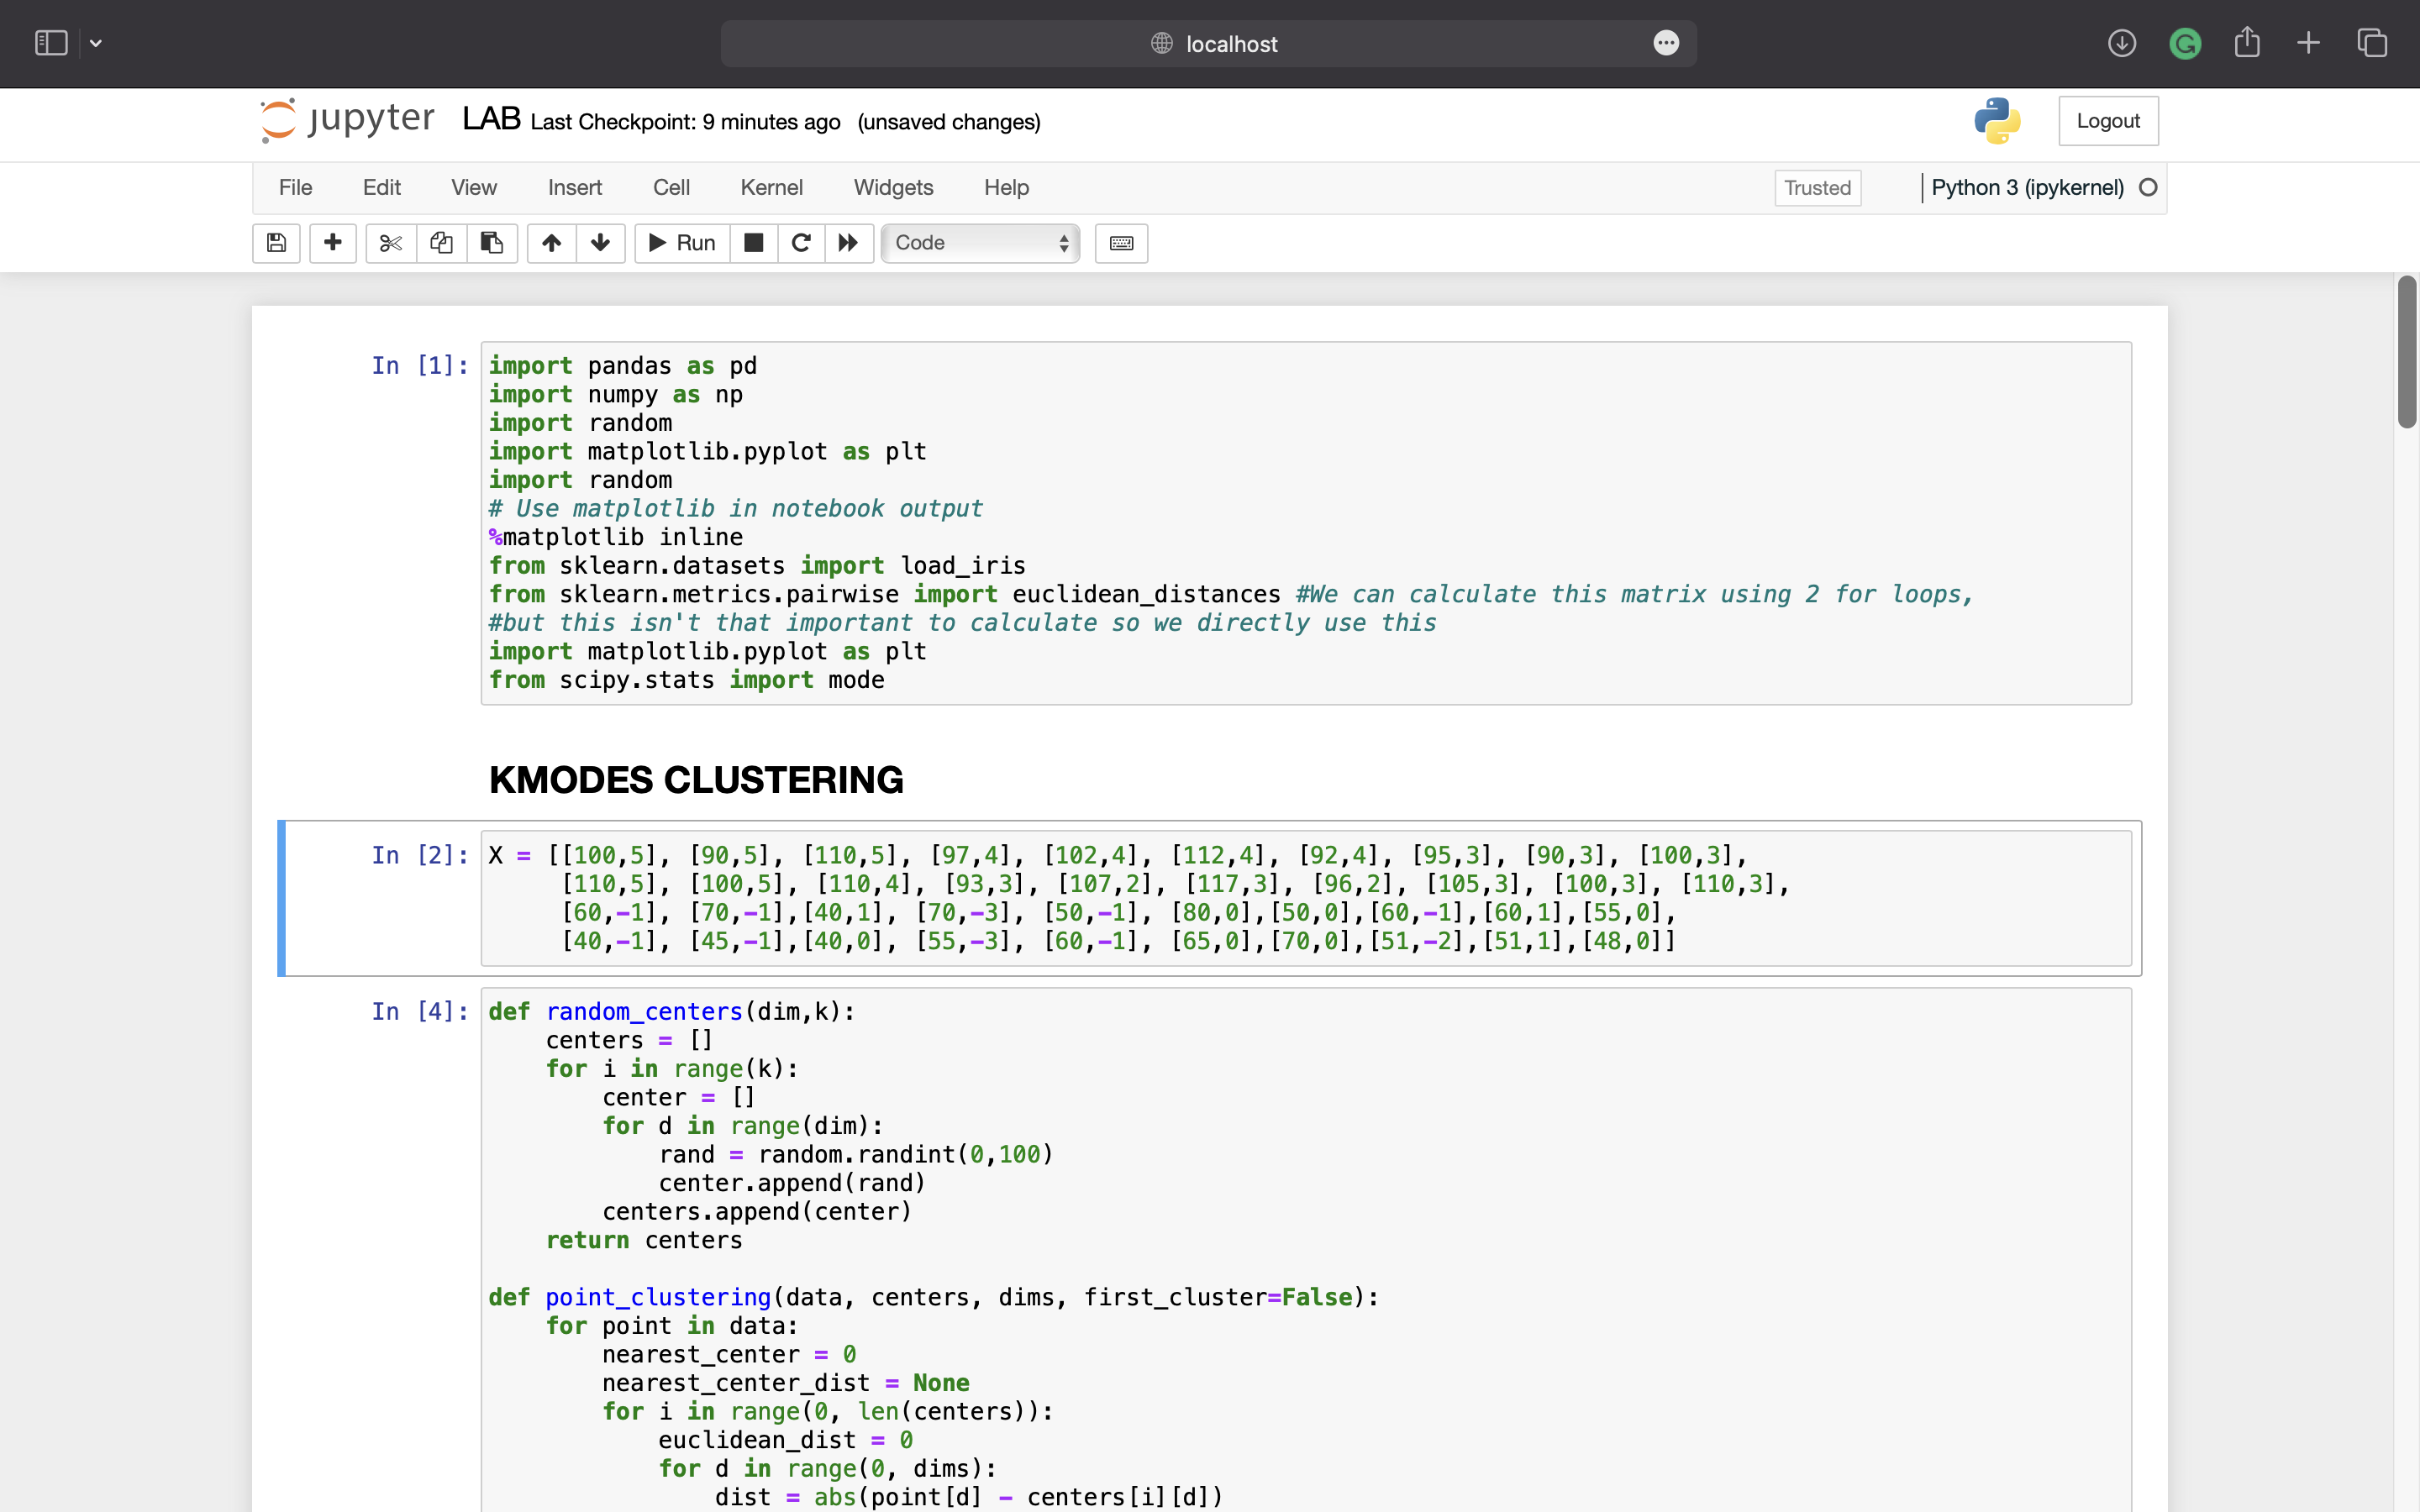
\includegraphics[scale=0.3]{images/1.png}
\section{KModes Clustering}
\subsection{Input - a 2D array}
\begin{lstlisting}[language=Python]
	def random_centers(dim,k):
	centers = []
	for i in range(k):
	center = []
	for d in range(dim):
	rand = random.randint(0,100)
	center.append(rand)
	centers.append(center)
	return centers
	
	def point_clustering(data, centers, dims, first_cluster=False):
	for point in data:
	nearest_center = 0
	nearest_center_dist = None
	for i in range(0, len(centers)):
	euclidean_dist = 0
	for d in range(0, dims):
	dist = abs(point[d] - centers[i][d])
	euclidean_dist += dist
	euclidean_dist = np.sqrt(euclidean_dist)
	if nearest_center_dist == None:
	nearest_center_dist = euclidean_dist
	nearest_center = i
	elif nearest_center_dist > euclidean_dist:
	nearest_center_dist = euclidean_dist
	nearest_center = i
	if first_cluster:
	point.append(nearest_center)
	else:
	point[-1] = nearest_center
	return data
	
	def mean_center(data, centers, dims):
	print('centers:', centers, 'dims:', dims)
	new_centers = []
	for i in range(len(centers)):
	new_center = []
	n_of_points = 0
	total_of_points = []
	for point in data:
	if point[-1] == i:
	n_of_points += 1
	for dim in range(0,dims):
	if dim < len(total_of_points):
	total_of_points[dim] += point[dim]
	else:
	total_of_points.append(point[dim])
	if len(total_of_points) != 0:
	for dim in range(0,dims):
	print(total_of_points, dim)
	new_center.append(total_of_points[dim]/n_of_points)
	new_centers.append(new_center)
	else: 
	new_centers.append(centers[i])
	
	
	return new_centers
	
	# Gets data and k, returns a list of center points.
	def train_k_means_clustering(data, k=2, epochs=5):
	dims = len(data[0])
	print('data[0]:',data[0])
	centers = random_centers(dims,k)
	
	clustered_data = point_clustering(data, centers, dims, first_cluster=True)
	
	for i in range(epochs):
	centers = mean_center(clustered_data, centers, dims)
	clustered_data = point_clustering(data, centers, dims, first_cluster=False)
	
	return centers
	
	def predict_k_means_clustering(point, centers):
	dims = len(point)
	center_dims = len(centers[0])
	
	if dims != center_dims:
	raise ValueError('Point given for prediction have', dims, 'dimensions but centers have', center_dims, 'dimensions')
	
	nearest_center = None
	nearest_dist = None
	
	for i in range(len(centers)):
	euclidean_dist = 0
	for dim in range(1, dims):
	dist = point[dim] - centers[i][dim]
	euclidean_dist += dist**2
	euclidean_dist = np.sqrt(euclidean_dist)
	if nearest_dist == None:
	nearest_dist = euclidean_dist
	nearest_center = i
	elif nearest_dist > euclidean_dist:
	nearest_dist = euclidean_dist
	nearest_center = i
	print('center:',i, 'dist:',euclidean_dist)
	
	return nearest_center
\end{lstlisting}

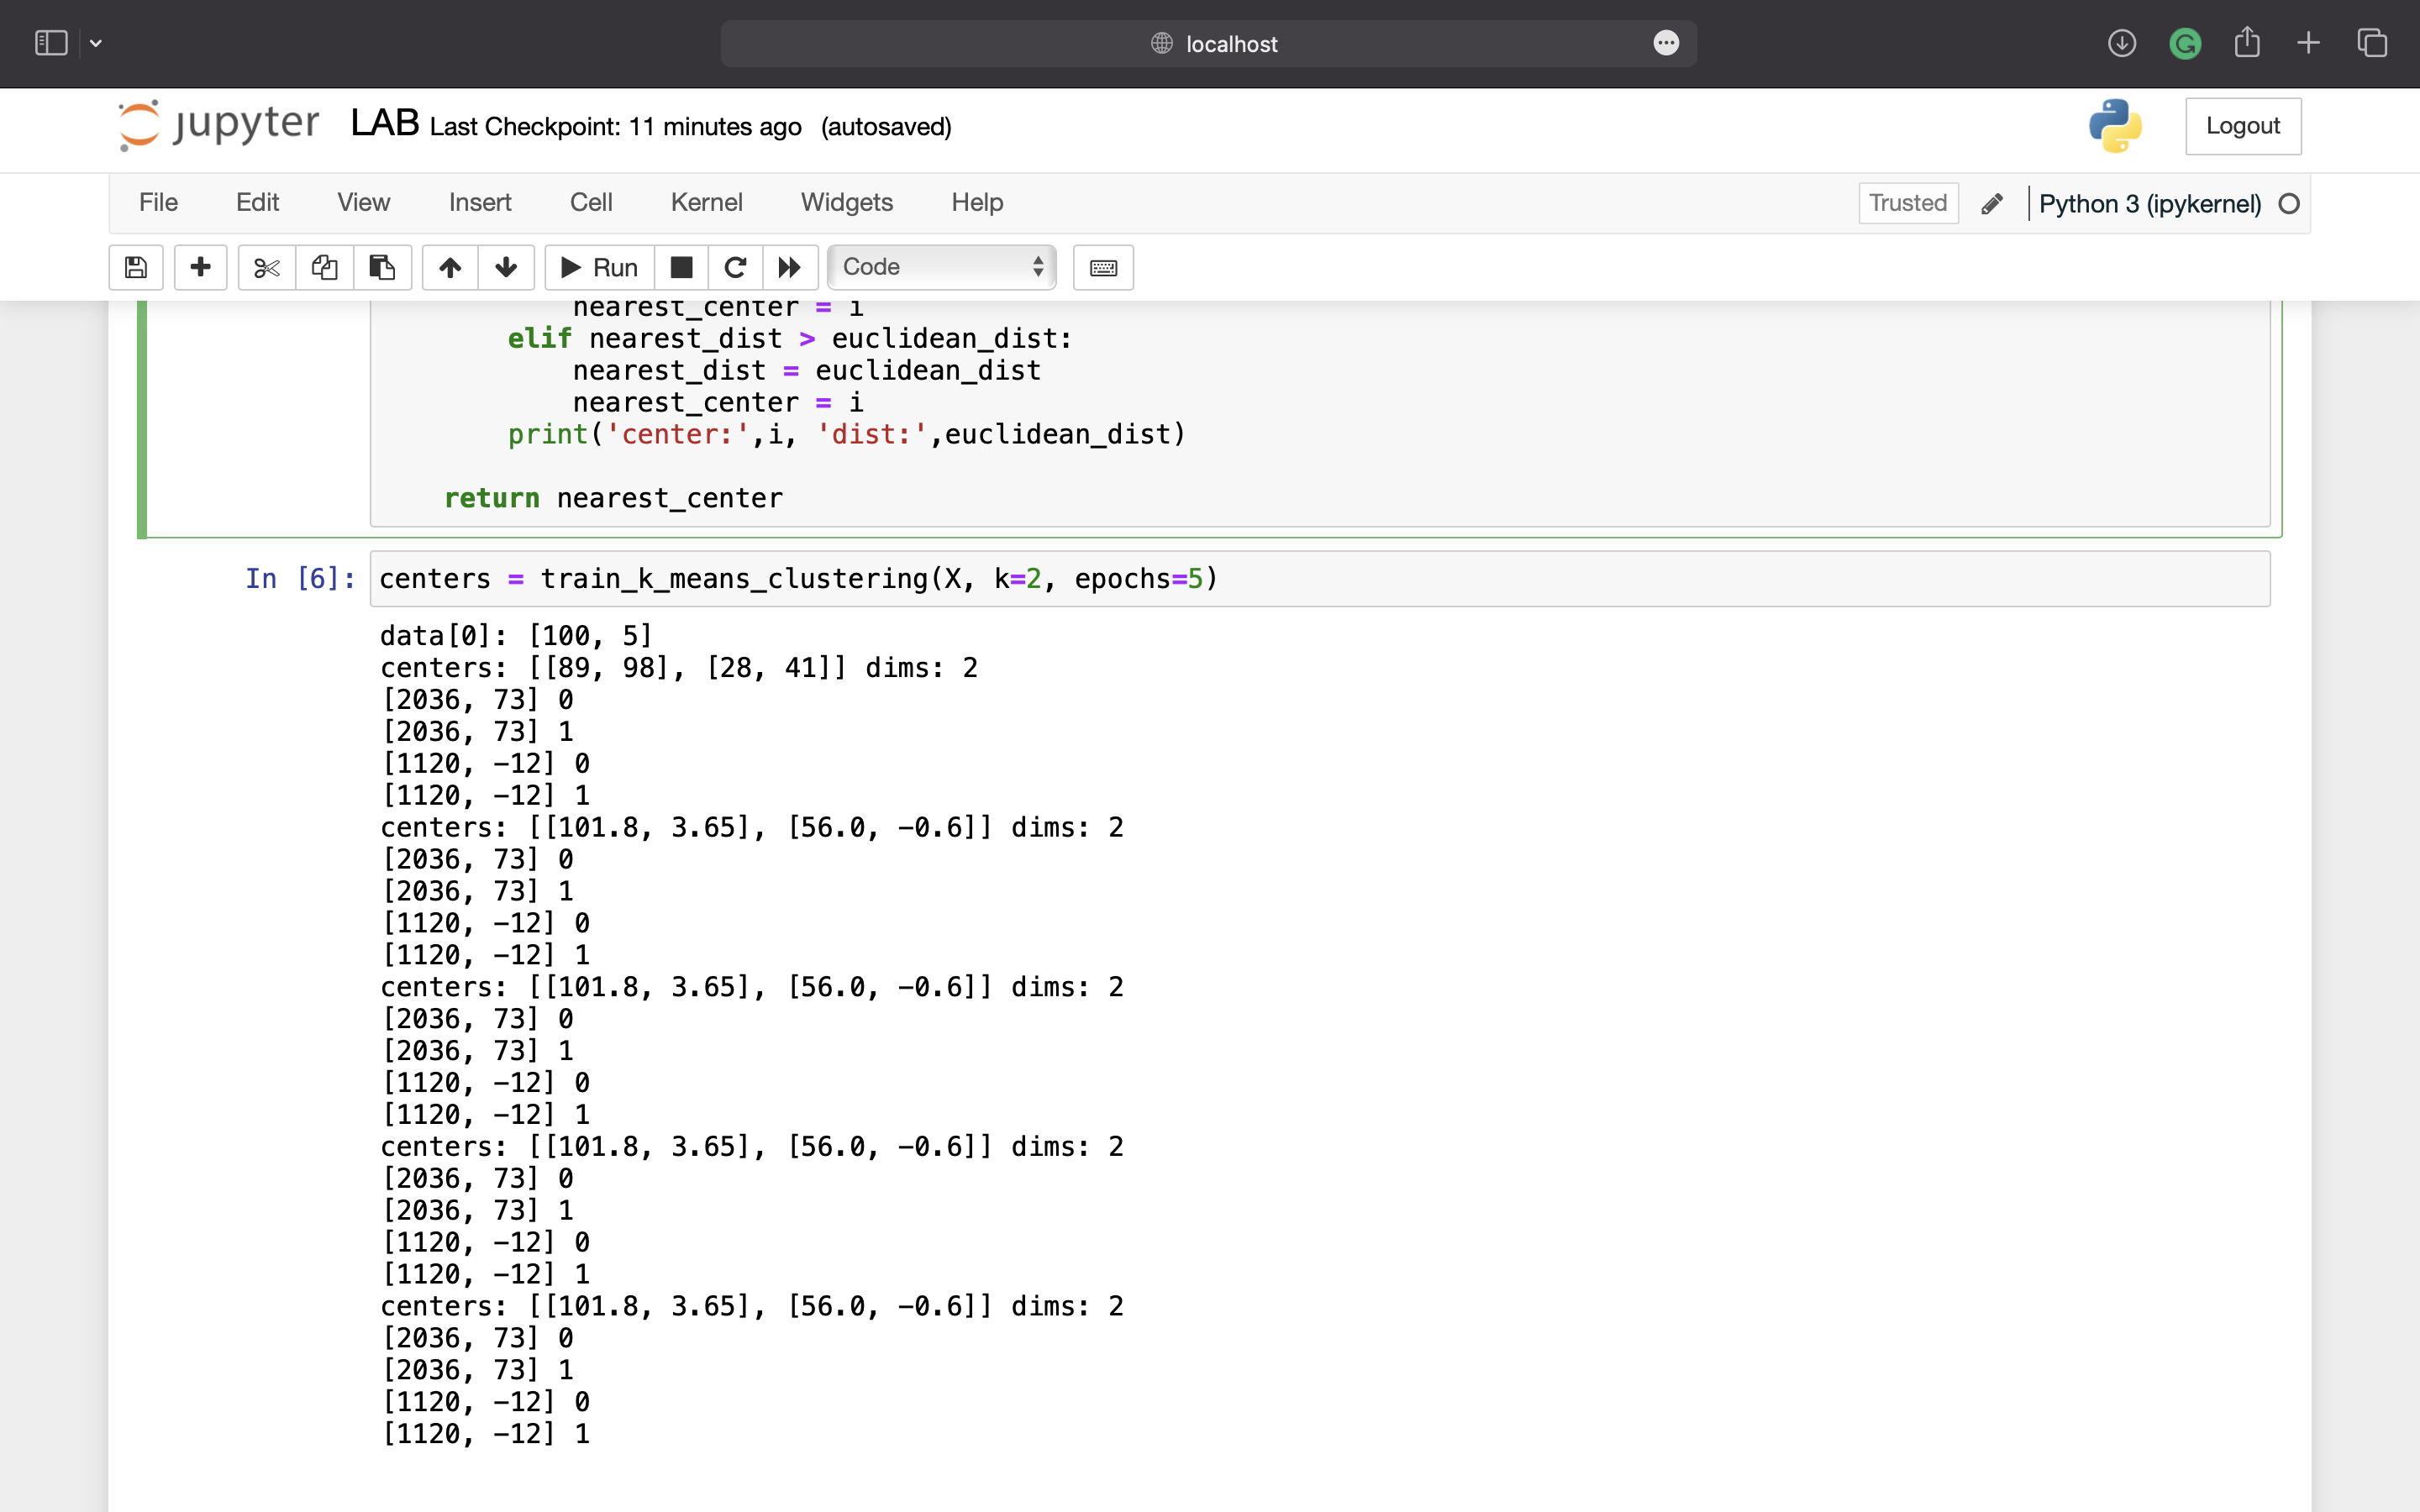
\includegraphics[scale=0.3]{images/2.png}
\section{KModes Clustering}
\begin{lstlisting}[language=Python]
	clusters = np.zeros(data.shape[0], dtype=int)
	clusters_prev = np.zeros(data.shape[0], dtype=int)
	
	
	for i in range(10):
	for j, object in enumerate(data):
	distances = np.array([sum(object != mode) for mode in modes])
	clusters[j] = np.argmin(distances)
	
	for j in range(k):
	modes[j] = mode(data[clusters == j]).mode[0]
	
	
	if (clusters == clusters_prev).all():
	break
	clusters_prev = clusters
	
	print("The cluster assignments for each data object: ", clusters)
	print("Modes for each cluster: ", modes)
	
\end{lstlisting}
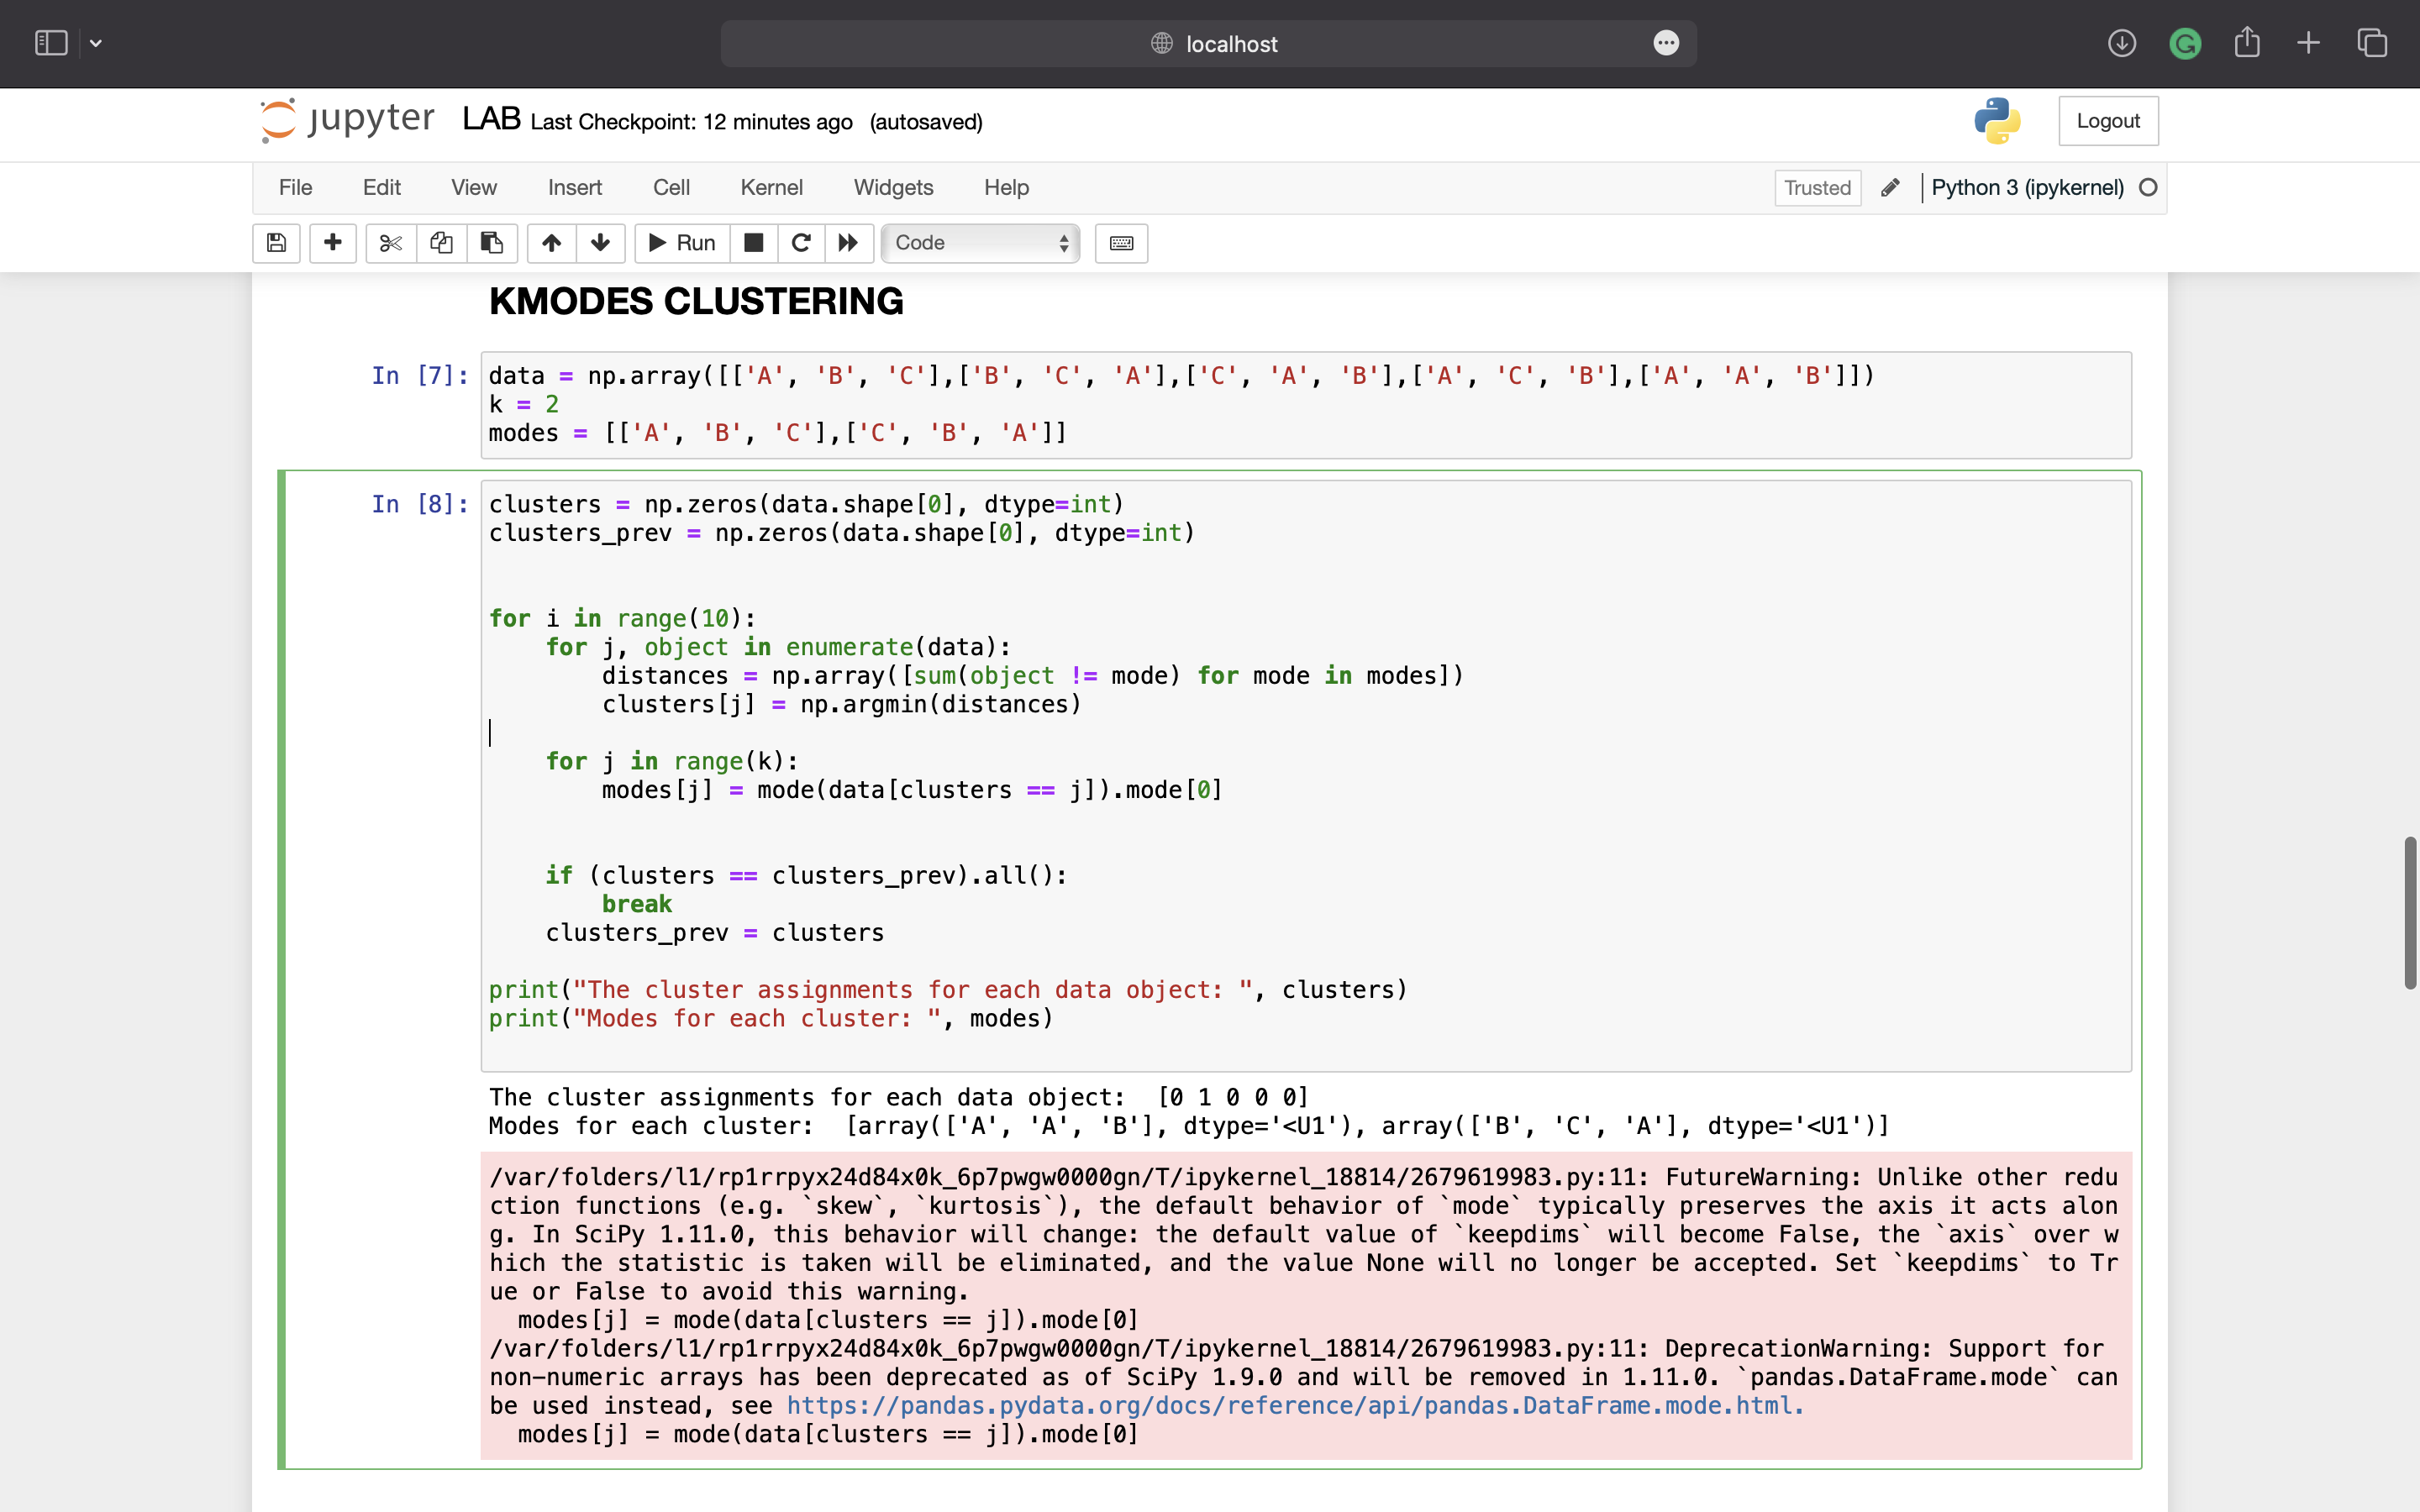
\includegraphics[scale=0.3]{images/4.png}
\section{Heirarchial Clustering}
\begin{lstlisting}[language=Python]
	def OwnHeirarchical(data, cutoff, linkage):
	#This is done using dynamic programming approach
	# if 1, it is single linkage else 2 is complete linkage, 3 is average linkage
	distance_matrix = euclidean_distances(data, data) 
	distance_matrix = np.tril(distance_matrix) 
	distance_matrix[distance_matrix == 0] = np.inf #Step 3 - Replace 0 by inf, it makes it easy for us to extract minimum using min function
	df = pd.DataFrame(data=np.ones(data.shape[0])*np.inf) #Initialized a dataframe which will store which point is in which cluster
	if cutoff > distance_matrix.shape[0]: #If user provides impractical cut-off, cluster everthing into one cluster and not listen to user 
	cutoff = distance_matrix.shape[0]
	if linkage == 1: #This 1 means formula of single linkage will be used, it is explained ahead
	d = {} #This dictionary keeps record of which data points or cluster are merging, hence can be used to make a dendogram
	for i in range(0,cutoff):
	ij_min = np.unravel_index(distance_matrix.argmin(), distance_matrix.shape) #from the distance matrix, get the minimum distance
	#np.unravel_index gives us the position of minimum distance. e.g. (0,4) is where minimum value is present in matrix.
	#This is what we need as in Hierarchical clustering, we merge the two pairs with minimum distance
	if i == 0:
	df.iloc[ij_min[0]] = 0
	df.iloc[ij_min[1]] = 0
	else:
	try:
	a = int(df.iloc[ij_min[0]])
	except:
	df.iloc[ij_min[0]] = i
	a = i
	try:
	b = int(df.iloc[ij_min[1]])
	except:
	df.iloc[ij_min[1]] = i
	b = i
	df[(df[0]==a) | (df[0]==b)] = i
	d[i] = ij_min
	
	for j in range(0, ij_min[0]):
	
	if np.isfinite(distance_matrix[ij_min[0]][j]) and np.isfinite(distance_matrix[ij_min[1]][j]):
	
	distance_matrix[ij_min[1]][j] = min(distance_matrix[ij_min[0]][j], distance_matrix[ij_min[1]][j])
	
	distance_matrix[ij_min[0]] = np.inf
	return d, df[0]
	elif linkage == 2:
	d_complete = {}
	for i in range(0,cutoff):
	ij_min = np.unravel_index(distance_matrix.argmin(), distance_matrix.shape)
	if i == 0:
	df.iloc[ij_min[0]] = 0
	df.iloc[ij_min[1]] = 0
	else:
	try:
	a = int(df.iloc[ij_min[0]])
	except:
	df.iloc[ij_min[0]] = i
	a = i
	try:
	b = int(df.iloc[ij_min[1]])
	except:
	df.iloc[ij_min[1]] = i
	b = i
	df[(df[0]==a) | (df[0]==b)] = i
	d_complete[i] = ij_min
	for j in range(0, ij_min[0]):
	if np.isfinite(distance_matrix[ij_min[0]][j]) and np.isfinite(distance_matrix[ij_min[1]][j]):
	
	distance_matrix[ij_min[1]][j] = max(distance_matrix[ij_min[0]][j], distance_matrix[ij_min[1]][j])
	distance_matrix[ij_min[0]] = np.inf
	return d_complete, df[0]
	elif linkage == 3:
	d_average = {}
	for i in range(0,cutoff):
	ij_min = np.unravel_index(distance_matrix.argmin(), distance_matrix.shape)
	if i == 0:
	df.iloc[ij_min[0]] = 0
	df.iloc[ij_min[1]] = 0
	else:
	try:
	a = int(df.iloc[ij_min[0]])
	except:
	df.iloc[ij_min[0]] = i
	a = i
	try:
	b = int(df.iloc[ij_min[1]])
	except:
	df.iloc[ij_min[1]] = i
	b = i
	df[(df[0]==a) | (df[0]==b)] = i
	d_average[i] = ij_min
	for j in range(0, ij_min[0]):
	if np.isfinite(distance_matrix[ij_min[0]][j]) and np.isfinite(distance_matrix[ij_min[1]][j]):
	
	distance_matrix[ij_min[1]][j] = (distance_matrix[ij_min[0]][j] + distance_matrix[ij_min[1]][j])/2.0          
	distance_matrix[ij_min[0]] = np.inf
	return d_average, df[0]
\end{lstlisting}
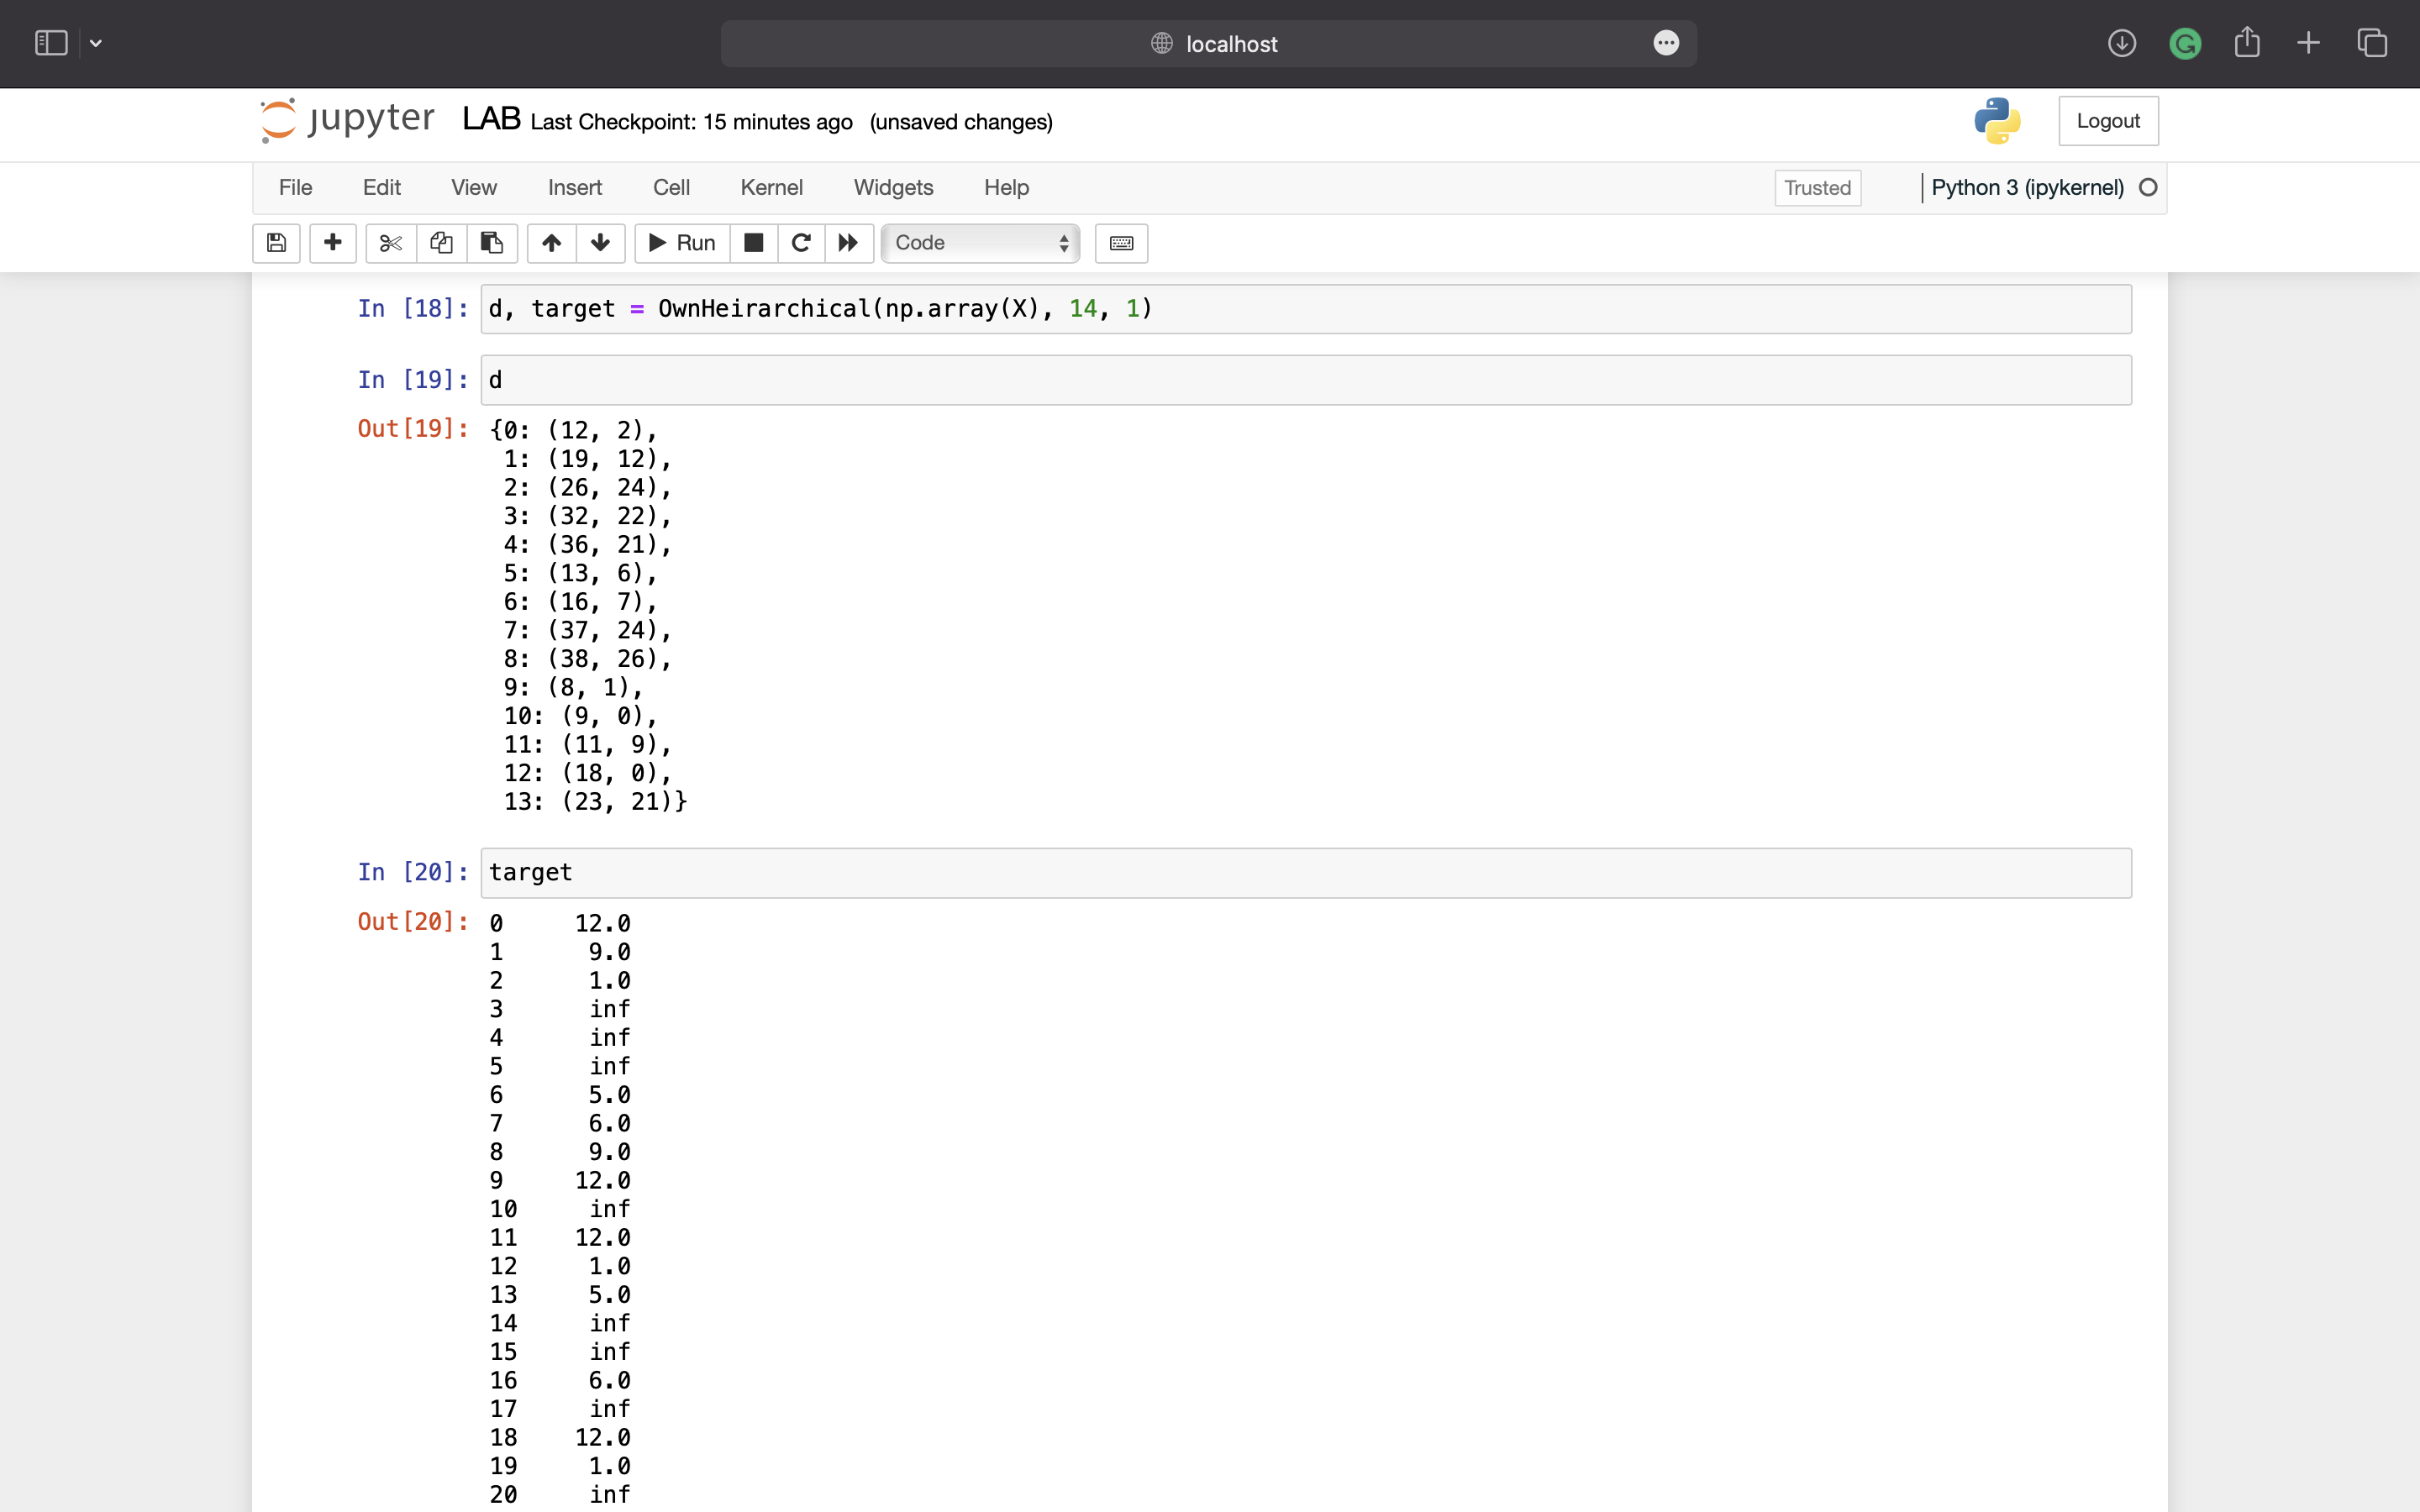
\includegraphics[scale=0.3]{images/5.png}\\\\\\\\\\\\
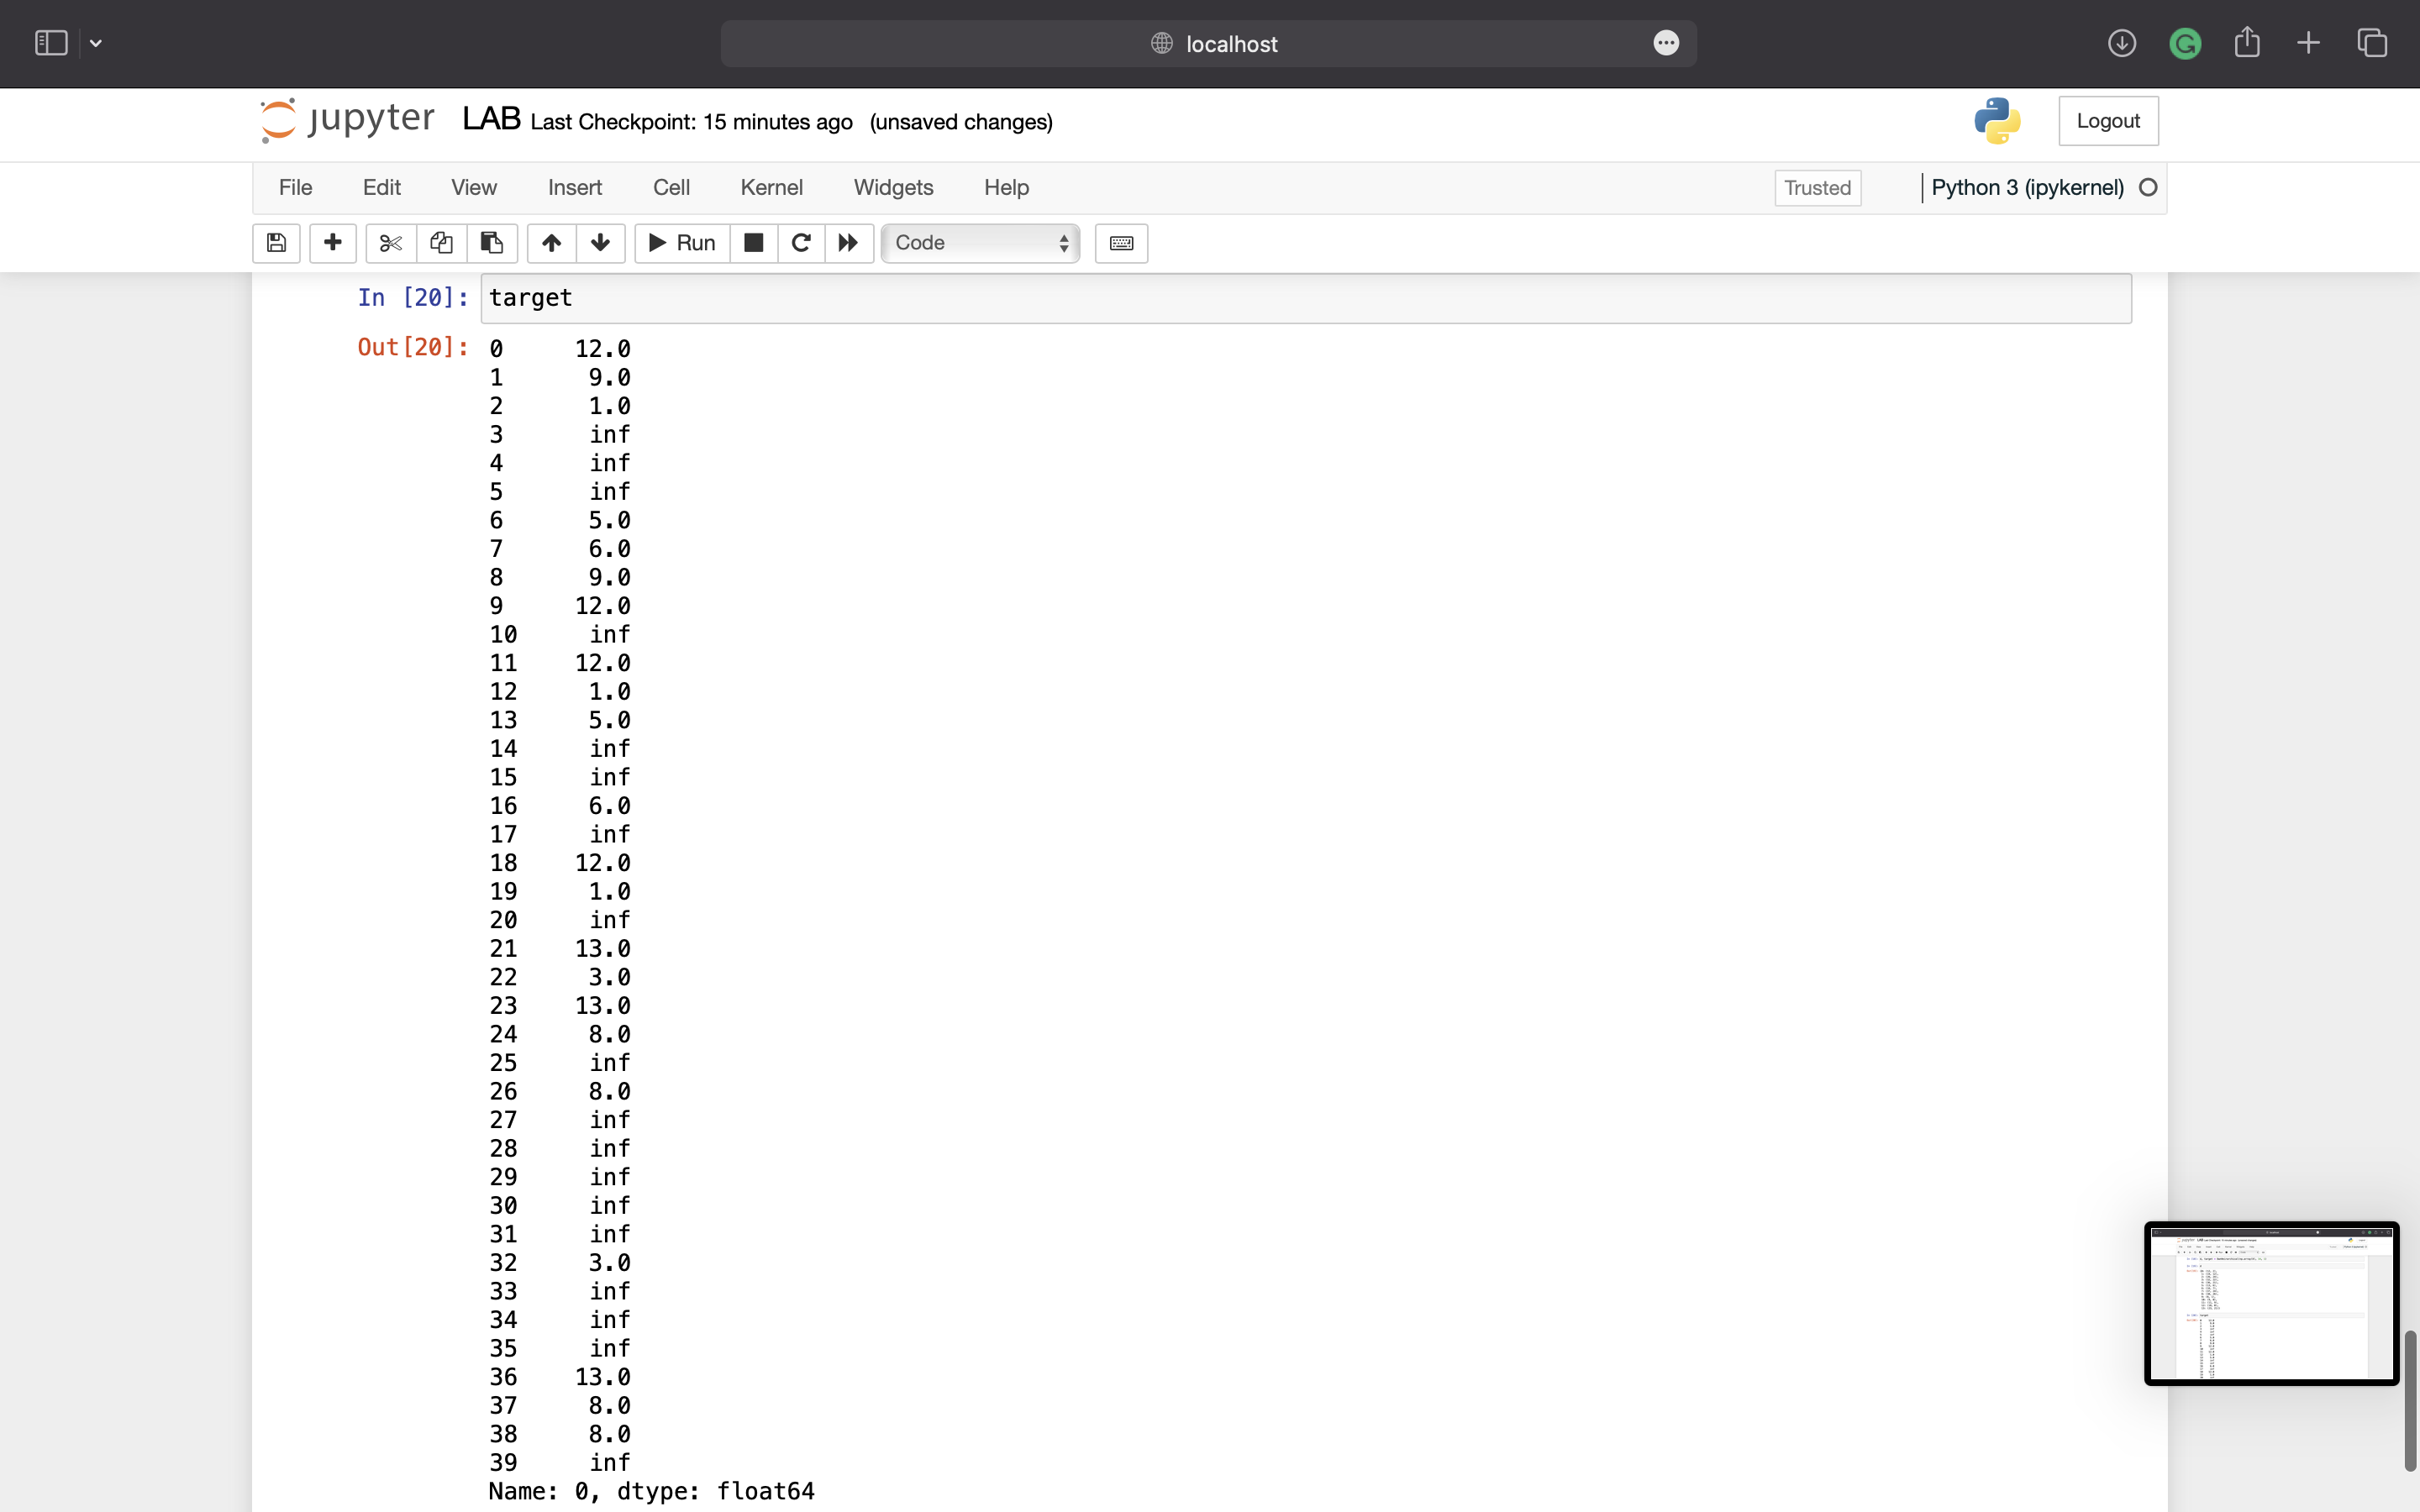
\includegraphics[scale=0.3]{images/6.png}
\end{document}